\chapter{Resoconto attività di verifica } \label{ResocontoAttivitàDiVerifica}
In questa sezione si riportano gli esiti, descritti ed analizzati, di tutte le attività$_{\scaleto{G}{3pt}}$ di verifica svolte.
\section{Revisione dei Requisiti}  \label{ResocontoAttivitàDiVerificaRevisioneDeiRequisiti}
Tutta la documentazione sviluppata nella prima fase da consegnare per la Revisione dei Requisiti ha subito una meticolosa ed attenta revisione da parte dei Verificatori. Questi ultimi hanno seguito, in questa attività$_{\scaleto{G}{3pt}}$, per ogni documento i metodi di \textit{Walkthrough$_G$} ed \textit{Inspection$_G$} relative all’analisi statica, stabilite nelle \textit{Norme di Progetto}. %% ?????? da rivedere quando scriviamo 3.4 sulle norme.
\subsection{Strategia adoperata per l’analisi statica dei documenti} \label{ResocontoAttivitàDiVerificaRevisioneDeiRequisitiStrategiaPerAnalisiStatica}
Il \textit{Verificatore} si è occupato di valutare la correttezza del documento, concentrandosi nell’individuare gli errori presenti in questo. Una volta individuati gli errori la strategia adottata è la seguente: 
\begin{itemize}
	\item Correzione degli errori sia ortografici che sintattici, non fedeli alle norme tipografiche fissate nelle \textit{Norme di Progetto v1.0.0}.
\end{itemize}

\subsection{Esiti verifica} \label{ResocontoAttivitàDiVerificaRevisioneDeiRequisitiEsitiVerifica}
Per ciascun documento stilato si è calcolato l’indice di Gulpease$_{\scaleto{G}{3pt}}$. I risultati sono mostrati qui di seguito.
Per evitare risultati errati nel calcolo di tale indice, non si sono tenuti in considerazione:
\begin{itemize}
	\item il frontespizio di ogni documento;
	\item le eventuali tabelle presenti nel documenti;
	\item i diari delle modifiche di ogni documento.
\end{itemize}

\quad
\def\tabularxcolumn#1{m{#1}}
{\rowcolors{2}{RawSienna!90!RawSienna!20}{RawSienna!70!RawSienna!40}	
	\begin{center}
		\renewcommand{\arraystretch}{1.4}
		\begin{tabularx}{11.65cm}{|c|c|c|}
			\hline
			\rowcolor{airforceblue}
			\textbf{Documento} & \textbf{Indice di Gulpease} & \textbf{Esito}\\
			\hline
			\textit{Analisi dei Requisiti v1.0.0} & 96  & \textit{Superato}\\
			\hline
			\textit{Norme di Progetto v1.0.0} & 75 & \textit{Superato}\\
			\hline
			\textit{Studio di Fattibilità v1.0.0} & 70 & \textit{Superato}\\
			\hline
			\textit{Piano di Progetto v1.0.0} & 77 & \textit{Superato}\\
			\hline
			\textit{Piano di Qualifica v1.0.0} & 80 & \textit{Superato}\\
			\hline
		\end{tabularx}
		\captionof{table}{\textbf{Elenco Indici di Gulpease$_{\scaleto{G}{3pt}}$ dei documenti versione v1.0.0}}
	\end{center}


\begin{figure}[!h]
	\begin{center}
		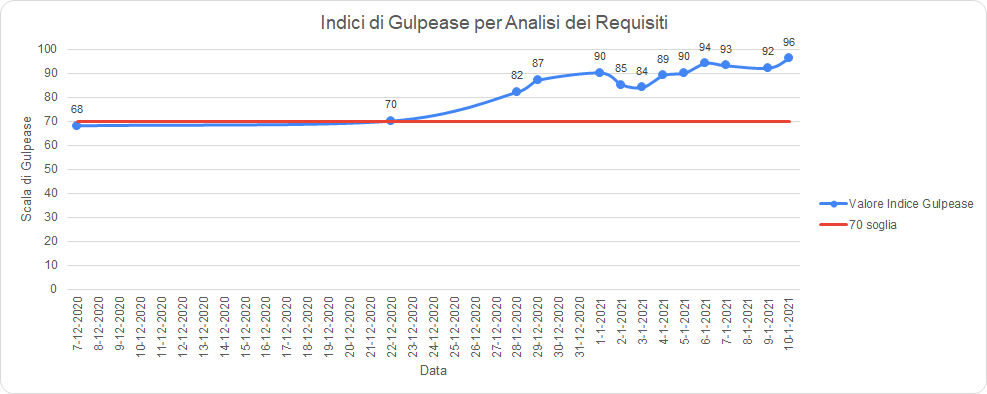
\includegraphics[width=1\linewidth]{../immagini/IndexGulpeaseAdR.png}
		\caption{\textbf{Andamento Indice di Gulpease$_{\scaleto{G}{3pt}}$ Analisi dei Requisiti}}
	\end{center}
\end{figure}

\begin{figure}[!h]
	\begin{center}
		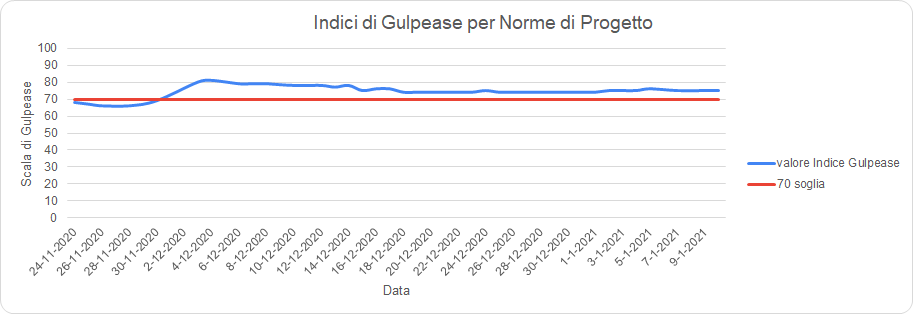
\includegraphics[width=1\linewidth]{../immagini/IndexGulpeaseNdP.png}
		\caption{\textbf{Andamento Indice di Gulpease$_{\scaleto{G}{3pt}}$ Norme di Progetto}}
	\end{center}
\end{figure}

\begin{figure}[!h]
	\begin{center}
		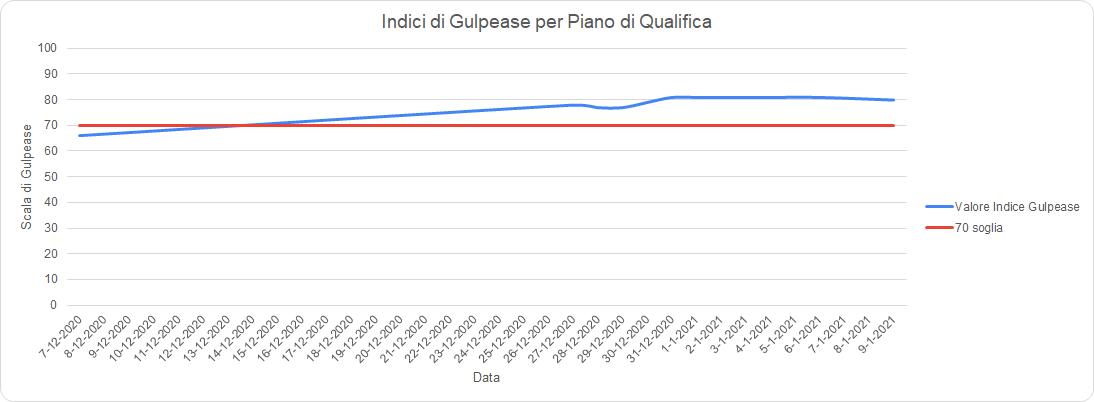
\includegraphics[width=1\linewidth]{../immagini/IndexGulpeasePdQ.png}
		\caption{\textbf{Andamento Indice di Gulpease$_{\scaleto{G}{3pt}}$ Piano di Qualifica}}
	\end{center}
\end{figure}

\begin{figure}[!h]	
	\begin{center}
		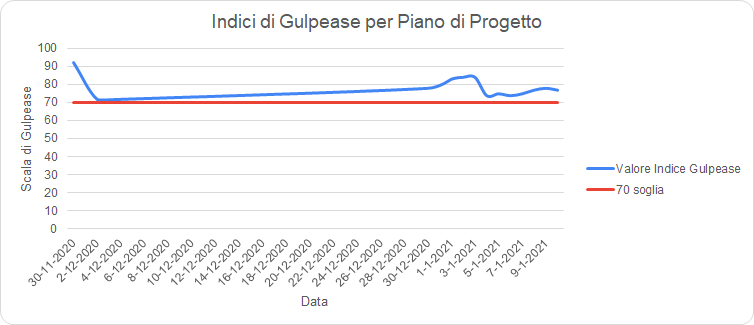
\includegraphics[width=1\linewidth]{../immagini/IndexGulpeasePdP.png}
		\caption{\textbf{Andamento Indice di Gulpease$_{\scaleto{G}{3pt}}$ Piano di Progetto}}
	\end{center}
\end{figure}

\begin{figure}[!h]
	\begin{center}
		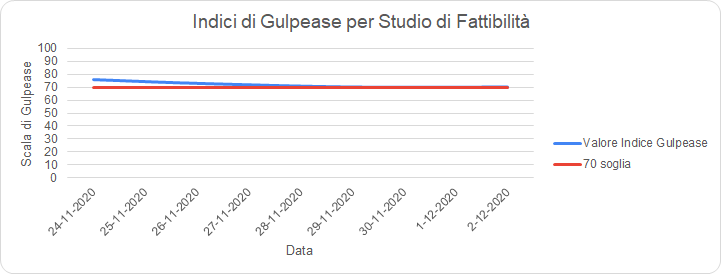
\includegraphics[width=1\linewidth]{../immagini/IndexGulpeaseSdF.png}
		\caption{\textbf{Andamento Indice di Gulpease$_{\scaleto{G}{3pt}}$ Studio di Fattibilità}}
	\end{center}
\end{figure}
\clearpage

Per quanto riguarda gli Indici di Gulpease$_{\scaleto{G}{3pt}}$ dei verbali si è deciso di rappresentare i risultati in forma tabellare.
Questo in quanto il verbale viene scritto tutta in una volta, quindi utilizzare un grafico temporale risulta non idoneo.
\quad
\def\tabularxcolumn#1{m{#1}}
{\rowcolors{2}{RawSienna!90!RawSienna!20}{RawSienna!70!RawSienna!40}	
	\begin{center}
		\renewcommand{\arraystretch}{1.4}
		\begin{tabularx}{11.65cm}{|c|c|c|}
			\hline
			\rowcolor{airforceblue}
			\textbf{Documento} & \textbf{Indice di Gulpease} & \textbf{Esito}\\
			\hline
			\textit{verbale\_interno\_28-10-2020} & 100  & \textit{Superato}\\
			\hline
			\textit{verbale\_interno\_19-11-2020} & 100 & \textit{Superato}\\
			\hline
			\textit{verbale\_interno\_24-11-2020} & 99 & \textit{Superato}\\
			\hline
			\textit{verbale\_interno\_04-12-2020} & 98 & \textit{Superato}\\
			\hline
			\textit{verbale\_esterno\_17-12-2020} & 99 & \textit{Superato}\\
			\hline
			\textit{verbale\_interno\_29-12-2020} & 100 & \textit{Superato}\\
			\hline
			\textit{verbale\_interno\_03-01-2021} & 100 & \textit{Superato}\\
			\hline
			\textit{verbale\_interno\_06-01-2021} & 100 & \textit{Superato}\\
			\hline
		\end{tabularx}
		\captionof{table}{\textbf{Elenco Indici di Gulpease$_{\scaleto{G}{3pt}}$ dei verbali versione v1.0.0}}
	\end{center}
